\chapter{The Saga of Overlapping Pulses}

Consider the waveform shown in Figure~\ref{fig:overlap}.
This is what was reconstructed by one specific channel.
``But wait'' I hear you say, ``overlapping pulses violates causality!''
This is correct, and \emph{why} this happened is the subject of this chapter.

\begin{figure}[htb]
  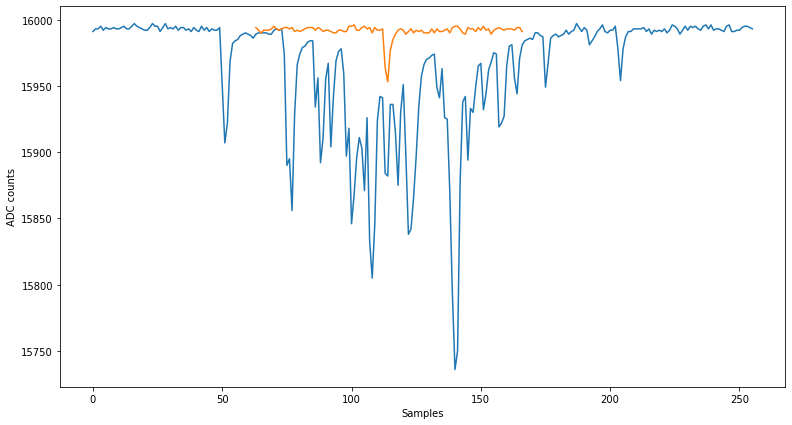
\includegraphics[width=\textwidth]{images/overlap_pulse}
  \caption{Overlapping pulses in one readout channel. Clearly something isn't working as expected.}\label{fig:overlap}
\end{figure}

Overlapping pulses clearly represent a problem of timestamp reconstruction, either on the digitizer or in the processing software.
This also presents a significant problem for the analysis.
Overlaps are instances where it is clear that a misreconstruction has happened, because it results in unphysical behavior that is easy to identify.
How often are timestamps being misreconstructed in such a way that it doesn't result in such easily-identifiable behavior?
The entire analysis depends on accurate timestamp reconstruction, because that's the basis on which peaks and events are built.
Getting two pulses to overlap is rather tricky, though, you have to hit a very narrow target.
Most of the time we aren't actually reading anything from a given channel.
We have \SI{1}{\micro\second} dark counts at around \SI{50}{\hertz} and \SI{10}{\micro\second} S2s at $\mathcal{O}(\mathrm{Hz})$.
This gives a ``live fraction'' of just under 1 part in $10^4$.
Thus, if timestamps are being misreconstructed, this is the chance that you'll see an overlap, or in other words, for each overlap you see, another $10^4$ misreconstructions happened that didn't result in overlaps, assuming normal conditions.

Clearly, this represents a problem for the analysis.
If photons get randomly moved around in time, this bodes ill for your threshold, because it'll turn a ``triggering'' 3-photon S1 into a ``non-triggering'' 2-photon S1.
The chance is much smaller that it turns a 2-photon S1 into a 3-photon S1, so if anything, your ``firmware-dino'' will manifest as the absense of a ``threshold-ino''.

\section{History}

Earlier in commissioning the NV had also been observing overlapping pulses.
For the NV it's a bit different, though, beacuse timestamp reconstruction for the V1730 is easier due to a 48-bit timestamp that only rolls over every couple of days.
At first we thought it was possible interplay between the length of a single photon waveform, the minimum pulse length the digitizer would return, and pre- and post-trigger settings, so that a few samples had actually been written out twice, but no.
A few rounds of feedback were done between CAEN and the NV DAQ people, and the problem went away.
Then we started seeing the same kinds of thing in the TPC data.

The exact details of when it first started are difficult to determine.
The conditions in the TPC were changing regularly for more than a year after it was installed.
What was inside it, how much was inside it, how much water was in the tank, what voltage was applied to the grids, what level of purity did the xenon have, etc.
It was also a very rare occurrence, only showing up maybe twice per week at most, so it's impossible to point to a specific change that might have precipitated something new happening.
The exact cause is still unknown but read on for some speculation on this.

\section{Symptoms}

A couple of things ended up being related to this issue in unexpected ways.

\subsection{Anomalous rates}

Sometime around late April or early May we started noticing strange things in the rate monitor.
The reader rates would briefly spike very high, but then didn't return to the original pre-spike values until the end of the run, remaining a factor of two or three higher than normal, as can be seen in Figure~\ref{fig:anomalous_rate}
However this effect could not be found by actually inspecting the \texttt{raw\_records} after the run.
The data on disk pre-spike and post-spike were basically the same, no significant change in rate in any channel could be observed.
Where did all this extra data come from?
Where did it go?
What was it?
No one knew, so we just changed the value reported to the website from the number of bytes read from the digitizers to the number of bytes written to disk.
\begin{figure}[htb]
  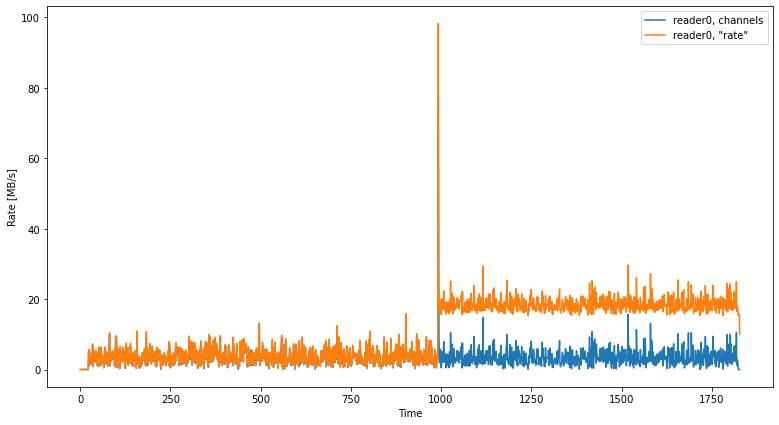
\includegraphics[width=\textwidth]{images/anomalous_rate}
  \caption{Despite this change in average rate, no effect could be seen in the data going to disk}\label{fig:anomalous_rate}
\end{figure}

\subsection{Double-storing data}

The strax-format data written to disk is a subset of what is read from the digitizers.
For the DPP-DAW firmware we basically ignore the event header and focus exclusively on the channel header.
The event header is still necessary because it tells us which channels are present, and things like word count which is useful for bookkeeping and navigating, but the values we actually write to disk are the timestamp and waveform found in the channel's payload.
We can reconstruct most of what was in the event header by grouping \texttt{raw\_records} into triggering events and working backwards, but some of the flags in the header are guaranteed to be lost, and also we can't reconstruct the event timestamp.
We figured out how we could store copies of both the raw unfiltered CAEN-format data without affecting the usual strax-format data necessary for live processing etc, in a way that didn't require undoing the reformatting process which technically is not lossless.
CAEN wanted this for for their efforts in digging into the issue.

An overlap eventually happened in a run where we were double-storing the data, so we duly gave them a few gigabytes of raw CAEN-format data, a channel number, and a rough measurement of where the overlap happened.
A bit later they came back with two questions (more, really, but these are the important ones).
First, they couldn't find the overlap, how sure were we it had happened?
Second, why were there so many events consisting of just the four-word event header?

\subsubsection{The Magic Number}

Indeed, upon manual inspection of the raw timestamps in the CAEN-format data, no overlap had occurred.
Strax disagreed.
However, by a painstaking process of manually looking for binary-identical pulses, an offset was found between the offending strax-format ``overlapping'' pulse and its corresponding CAEN-format version of exactly \SI{21.47}{\second}.
The reader has doubtless already recalled the discussion of this magic DAQ number from Section~\ref{sec:v1724}.
Anytime this number shows up in the data, shenanigans were involved.

\subsubsection{Empty events}

Also evident in this run was a very interesting trend of event sizes.
Most (and by ``most'' I mean $>99\%$) of the events read out by this digitizer only consisted of the 4 words that form the event header.
A whopping 15~million events were entirely missing any actual waveform payload.
This run was only half an hour long, and the first half didn't have any of these.
This half-gigabyte of data represents a non-trivial portion of the entire 2.7-ish gigabytes that board read during this run.

Upon inspection of the logs for this run, more shenanigans were discovered.
For most of the run, this board had reported a status of \texttt{0x81bc}.
A lot of other boards also reported this, including some of the HE boards, which really shouldn't ever go busy.
Normally, if one board reports \texttt{0x81bc} for any sustained interval, it's usually the AM, and all the other boards report \texttt{0x181a4}.
I think once or twice I've seen \texttt{0x181bc} but that's a very transient state that only sticks around for a few milliseconds on average.
Point is, if we have a sustained busy, we should see that represented in both the board status and the data rate.
We didn't see any difference in either, so does this mean that the BUSY wasn't issued, the VETO wasn't issued, or the VETO was ignored?
For this we turn to the AM data, which contained two BUSY STARTs and one BUSY END.
The matched pair corresponded to an interval of some \SI{300}{\milli\second}, and the unmatched BUSY START happened shortly after this interval.
The logic whereby we issue a VETO is so simple as to be bullet-proof (see Section~\ref{sec:busyveto}), and we see that the V1495 received a BUSY and issued a VETO.
The boards, however, seem to have missed the memo.

To thicken the plot, even though many boards were reporting sustained BUSYs, every single digitizer was still reporting clock rollovers as usual.
No missed rollovers were reported, everything lined up.
However, the number of readout cycles between rollovers was reduced.
We log the digitizer status every $10\,000$ readout cycles, which normally takes about one second, so generally there are 18-20 log statements per digitizer between rollovers.
Here, however, we were seeing only two or three.
This slowdown means that the readout threads were spending more time pulling data from digitizers than sleeping, so clearly data was being collected from somewhere.

It was during this extended interval, when a VETO had been issued but was largely being ignored, that the pulse overlap happened.
On one hand any events would be removed from the analysis because a VETO was issued, but on the other hand this clearly represents unwanted behavior on the part of the digitizers.
While we were figuring this out, CAEN came back with a new firmware version which contained a fix for an issue they had found relating to how boards handed the BUSY condition.
This seems to line up with the issue we had been finding where the boards weren't responding properly to a VETO following a particular BUSY condition.
We hope that this means the core issue was identified, and the firmware fix effective.

The problem with fixing rare bugs is that it's hard to prove that the bug has been squashed when you aren't the one squashing it.
We observed 17 such overlaps between the start of July and the end of September 2021, which is a rate of \SI{0.18}{\per\day}.
If you don't see an overlap for two weeks, that isn't even a two-sigma effect.
A month gets you to three sigma.

\section{Commentary}

So what was actually the root cause here?
It's difficult to concretely say without being able to step through the digitizer logic, but we can make some educated guesses based on what we observed and what CAEN said.
We saw that these periods of ``anomalous readout'' where the boards were supposed to be under a VETO followed a very large rate spike and a period of a normal BUSY.
If a muon punches through both the top and bottom stack of the TPC, this is the largest signal the TPC can ever see.
If the purity is very good then the electron cloud won't attenuate much over the length of the detector.
This will be an S2 that puts every low-energy channel (and probably most high-energy channels) above threshold for at the very least one drift length, which is a sizeable fraction of the digitizer's memory.
So, most if not all boards should reach full saturation where literally all of the board's memory is filled.
We see this as a massive rate spike (again, see Figure~\ref{fig:anomalous_rate}) and a few hundred milliseconds of BUSY while we try to read several hundred megabytes from all the digitizers.

However, the digitizers don't properly recover from being completely filled, and they stop responding to the VETO signal that the V1495 tries.
The boards, meanwhile, are losing their shit and ``recording'' a huge number of header-only events because they don't have any memory available to actually store waveforms (the irony being that the sheer number of header-only events was probably a major contributor to this problem).
Redax reads all these events out, but you without any actual content in the event payload none of it goes to disk, and because these events are coming at such a large rate we don't see it in the BLT report at the end of a run.
A block transfer consisting of only one header-only event is highly suspicious, but if there are hundreds waiting on the board then it's the same number of bytes being transferred as for ``good'' data and so you won't see it with the amount of metadata we usually store.
In this period of non-standard operation we can't really rely on the timestamps being reliable, so it shouldn't really be a surprise if we happen to misreconstruct a timestamp in an interval where we shouldn't be seeing any data at all.

